\documentclass[twocolumn,a4paper]{IEEEtranfr}
\usepackage[utf8]{inputenc}
\usepackage[utf8]{inputenc}
\usepackage{multicol}
\usepackage[french]{babel}
\usepackage[T1]{fontenc}
\usepackage{natbib}
\usepackage{verbatim}
\usepackage{graphicx}
\usepackage{url}
\usepackage[export]{adjustbox}
\usepackage[fleqn]{amsmath}
\usepackage{multicol}
\usepackage{lipsum}
\usepackage{placeins}
\usepackage{caption}
\usepackage{nameref}

\title{Amélioration de l'ordonnancement des résultats dans un moteur de recherche}
\author{Baptiste \textsc{Aden}, Jordan \textsc{Bachelin}, Pierre-Henri \textsc{Collin}, Kévin \textsc{Ledy}, Haozhi \textsc{Li}}

\begin{document}

\maketitle

\begin{abstract}
L'objectif du projet est de démontrer l'efficacité d'une technologie de machine learning dans un moteur de recherche Apache Solr. La première étape a été de se familiariser au logiciel et à son environnement. Ensuite, des données de test personnalisées ont été générées. Puis, un choix de technologie de machine learning a été fait : Learning to Rank (LTR), plugin directement intégré au logiciel dans sa dernière version. Enfin, la comparaison des classements sans et avec plugin a mis en évidence l'efficacité du machine learning : LTR prend en compte les statistiques d'usages afin de proposer un nouveau classement plus pertinent.
\end{abstract} 

\begin{keywords}
Moteur de recherche, classement et pertinence des résultats, machine learning, Big Data
\end{keywords}

\section{Introduction}
Face à de grands volumes de données, le classement des résultats a un rôle capital dans un moteur de recherche pour répondre aux attentes de l'utilisateur. Dans Apache Solr, chaque résultat de requête se voit attribué un score déterminant sa place dans le classement. De base, ces scores sont égaux à la fréquence des termes de la requête dans l'ensemble des documents de la base de données indexées \cite{docTFIDF}. Cependant, la plupart du temps, des règles vont également être définies manuellement pour améliorer la pertinence du classement : un résultat respectant une règle verra son score (et donc sa place dans le classement) augmenter. Ce classement doit sans cesse rester pertinent, ainsi les administrateurs vont être amenés à ajouter des règles supplémentaires au cours du temps. À terme, cela devient difficile à maintenir car celles-ci peuvent entrer en conflit, ce qui peut entraîner de lourdes modifications pour un simple ajout.

L'objectif du projet est de réaliser un prototype de moteur de recherche utilisant le \textit{machine learning} et de comparer les classements de résultats avec et sans son utilisation. Cette technologie vise à améliorer la pertinence de classement des résultats de recherches et à rendre sa maintenance plus aisée. En fonction des résultats obtenus, Jouve sera éventuellement amené à mettre cela en place pour améliorer son propre service client.

Dans cet article seront alors précisées dans un premier temps les problématiques abordées, les méthodes employées pour y faire face, puis viendront les résultats obtenus grâce à la démarche mise en oeuvre. La conclusion apportera enfin un point de vue critique sur l'ensemble du déroulement de ce projet.

\section{Méthodes, matériels et moyens}

\subsection{Méthodologie}

Tout d'abord, une méthodologie de travail agile a été choisie pour réaliser ce projet. En effet, celle-ci est largement utilisée chez Jouve et très pratique dans le cadre de ce projet, qui a par conséquent été découpé en trois sprints :\\
\begin{itemize}
  \item \textbf{Sprint 1 - Familiarisation avec le projet :} cette phase a consisté en la mise en place de l'environnement général (GitHub, Google Drive, etc.) et à la formation au moteur de recherche Apache Solr. Ainsi, cela a permis de mieux comprendre en quoi consistaient les règles de classement. Certaines ont été écrites et testées sur les données créées et utilisées tout au long de ce projet. En effet, pour se rapprocher au plus de l'utilisation qu'en fera Jouve, ces données représentent une base de vêtements qui pourrait être celle par exemple d'un site e-commerce. L'intérêt est double ici : d'une part, les données créées sont authentiques car inspirées d'un vrai site e-commerce (Amazon). D'autre part, les vêtements sont un type de données parlant pour tout le monde, ce qui est un avantage en cas de démonstration ou de soutenance orale. Le format JSON (JavaScript Object Notation) a été utilisé pour créer les différents vêtements (documents) de cette base.
  \begin{figure}[htpb]
    \begin{center}
        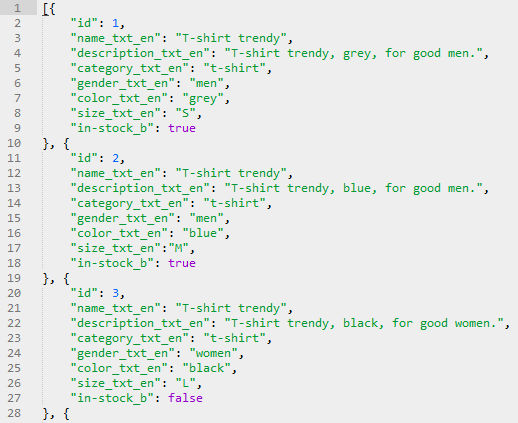
\includegraphics[width=7cm]{clothes.png}
    \end{center}
    \caption{Extrait de données JSON de vêtements \textbf{[SCREEN TO CHANGE + COMMENTER OU SUPPRIMER]}}
    \label{clothes}
  \end{figure}
  
  \item \textbf{Sprint 2 - Comparaison d'algorithmes :} il s'agit du sprint principal. Initialement, la première tâche de ce sprint était de comparer le plugin \textit{Learning to Rank} (LTR) avec les outils présents dans Apache Solr en recherchant dans la littérature et en en faisant l'expérience. En effet, bien que LTR soit dédié au ré-ordonnancement de résultats, il était nécessaire de s'assurer qu'il était aussi rentable de l'utiliser : installation sans trop de complications, utilisation intuitive, documentation disponible, etc. Cependant, après la fin du sprint 1, une nouvelle version du logiciel est sortie, intégrant directement le plugin et accompagnée d'une documentation en ligne régulièrement mise à jour. Le choix de son utilisation par le client a donc été rapidement proposé.
  
  La seconde tâche consista alors à apprendre à utiliser LTR. Pour ce faire, il a été nécessaire d'avoir recours à la documentation en ligne ainsi qu'aux différents exemples fournis pour réordonner des données selon de simples critères.\\
  
  
  \item \textbf{Sprint 3 - Finalisation :} une tâche majeure de ce sprint a été la réalisation d'une application web. Dans un premier temps, son rôle était uniquement de générer les données nécessaires en entrée du plugin (\textit{cf.} ci-après, sous-section \ref{ssec:ltr}). Dans un second temps, cette application permet également de comparer le classement de résultats obtenus avant et après ré-ordonnancement par LTR.
  
  Cinquante nouveaux documents ont également été créés afin de compléter la base de départ et ainsi observer les différences quant aux résultats et scores obtenus sur différentes requêtes pré-sélectionnées. Des statistiques ont été produites ensuite sur ces documents pour connaître le panel des différents types de vêtements, des différentes tailles, couleurs, etc. présentes dans cette base et ainsi appréhender les scores qu'il est possible d'obtenir avant d'utiliser le plugin LTR.
  
  A part cela, ce sprint a constitué principalement la partie livrables de ce projet. En effet durant cette période, il a été demandé de rendre compte auprès des tuteurs des résultats obtenus pour ce projet industriel. Il consistait donc notamment à la création de cet article scientifique mais également d'un poster reprenant ce qui est restitué ici de manière vulgarisée et plus concise cette fois-ci. Il fût très important pour celui-ci que l'objectif et les résultats de ce projet soit rapidement compris de tous (étudiants, professeurs, professionnels, intervenants, personnels, etc.) car il est très probable que ce poster soit affiché et consulté dans le hall de l'ESIR (École Supérieure d'Ingénieurs de Rennes) dans un futur proche.\\
\end{itemize}

Par ailleurs, Une réunion physique était planifiée toute les deux semaines chez Jouve afin de rendre compte à l'entreprise de l'avancement. Cela permettait d'alterner entre phase de familiarisation avec les technologies et phase de validation, car les encadrants professionnels ont une bonne connaissance d'Apache Solr.


\subsection{Learning to Rank}\label{ssec:ltr}

LTR agit sur les listes de résultats obtenues en réponse des requêtes pour ré-ordonner le classement et en améliorer la pertinence. L'action se déroule sur le \textit{top-N} des documents, c'est-à-dire les \textit{N} documents ayant les scores les plus élevés, avec \textit{N} défini manuellement. Cela permet de maintenir une latence faible et d'adapter son moteur de recherche à son besoin. En effet, selon le type et le volume des données, l'utilisateur parcourra un nombre variable de résultats (très rarement l'intégralité).

Le plugin s'appuie sur divers éléments pour fonctionner : 
\begin{itemize}
  \item \textbf{Le "model"} liste un ensemble de features et attribue à chacune un poids qui servira au ré-ordonnancement des résultats.
  \item \textbf{Les "features"} sont de nouvelles règles définissant ce sur quoi le plugin doit se baser pour modifier le score d'un résultat.
  \item \textbf{Les "training data"} sont des statistiques d'usages (d'un site e-commerce par exemple) qui permettent d'appréhender le comportement des utilisateurs. En reprenant l'algorithme \textit{RankSVM} \cite{rankSVM}, elles sont utilisées pour déterminer le poids à accorder à chaque feature dans les models, qui seront générés automatiquement.
\end{itemize}


\subsection{Démarche de test}

Pour vérifier l'efficacité de LTR, une démarche a été mise en place et utilisée à plusieurs reprises :
\begin{enumerate}
  \item \textbf{Génération des training data} avec l'application web. Ne disposant pas de statistiques d'usages réelles, l'application permet d'en créer des personnalisées en se basant sur le jugement humain. Pour ce faire, après avoir réalisé une requête, il faut attribuer subjectivement une note à chaque résultat, ce qui générera un fichier de statistiques.
  \item \textbf{Création du fichier de features}, décrivant les règles sur lesquelles le plugin doit se baser pour modifier les scores.
   \item \textbf{Comparaison des classements Solr sans et avec LTR}. D'une part, s'assurer que le nouveau classement proposé par le plugin respecte bien les données fournies en entrée. D'autre part, s'assurer que le nouveau classement est effectivement plus pertinent que l'ancien 
\end{enumerate}

La section \ref{sec:results} reprend cette démarche en utilisant des données d'exemples.


\section{Résultats}\label{sec:results}

\subsection{Training data}
\textbf{[SCREEN TRAINING DATA]}

\subsection{Features}
\textbf{[??? SCREEN MODEL ET FEATURES ???]}

\subsection{Comparaison avec Solr seul}
\textbf{[SCREEN RESULTS SOLR / RESULTS LTR]}



\section{Analyse et discussion}
\textbf{[TODO]}

\section{Conclusion}
\textbf{[TODO]}



\bibliographystyle{unsrt}
\bibliography{ref}

\end{document}
